
\section{附录：一维\trCompact\trManifold{}的分类}
\label{sec:appendix-dim1-classification}

\subsection{\trManifoldWithBoundary{}上的\trMorseFunction{}与\trAdapted{}\trVectorField}
\label{subsec:morse-functions-adapted-fields}

\setcounter{figure}{27}

现在让我们来考察一个\trManifoldWithBoundary{} $V$。我们固定一个定义在 $V$ 内、$\partial V$ 的某个邻域中的\trVectorField{} $X$，并假定它是\textbf{\trIncoming}（incoming）的，也就是说，对每一张\trChart{} $\varphi\colon U\to V$（这里 $U$ 是 $\RR^n$ 中半空间 $x_n\le 0$ 的一个\trOpen{}子集）与每一个 $x\in\partial V\cap\varphi(U)$，都有
\[
T_{\varphi^{-1}(x)}\varphi^{-1}(X_x)=\sum_{i=1}^{n}a_i\frac{\partial}{\partial x_i}\qquad\text{其中 } a_n\bigl(\varphi^{-1}(x)\bigr)<0\text{。}
\]

\begin{figure}[htbp]
\centering
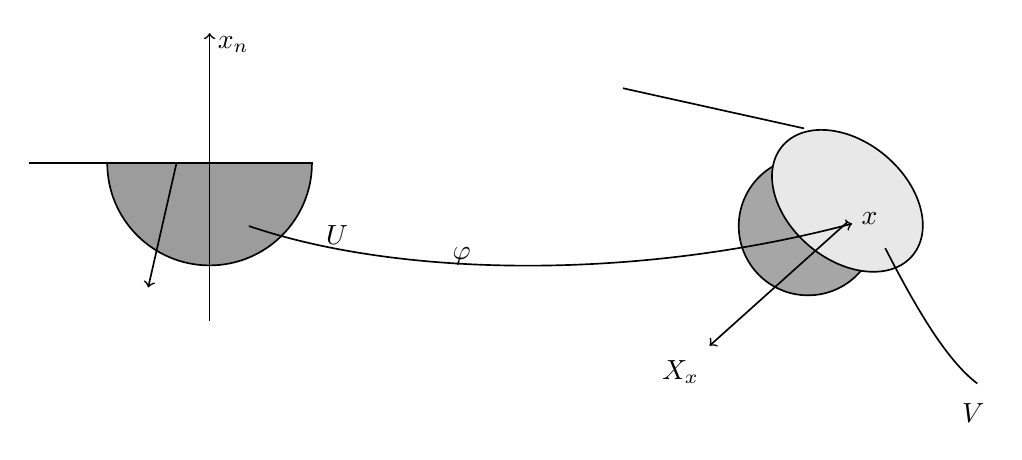
\begin{tikzpicture}[line width=0.6pt]
  \filldraw[fill=gray!78,line width=0.6pt] (-1.3,0.3) arc[start angle=180,end angle=360,radius=1.3] -- cycle;
  \draw (-2.3,0.3) -- (1.28,0.3);
  \draw[->] (0,-1.7) -- (0,1.95);
  \node at (0.3,1.8) {$x_n$};
  \draw[->] (-0.42,0.3) -- (-0.78,-1.28);
  \node at (1.62,-0.62) {$U$};
  \begin{scope}[shift={(7.6,-0.5)}]
    \filldraw[fill=gray!70,line width=0.6pt] (0,0) circle (0.88);
    \filldraw[fill=gray!18,line width=0.6pt]
      (0.5,0.32) ellipse[x radius=1.08,y radius=0.75,rotate=-40];
    \draw (-2.35,1.75) -- (-0.05,1.24);
    \draw (0.98,-0.28) .. controls (1.35,-1.0) and (1.75,-1.7) .. (2.15,-2.0);
    \node at (0.78,0.1) {$x$};
    \draw[->] (0.5,0.05) -- (-1.25,-1.52);
    \node at (-1.62,-1.85) {$X_x$};
    \node at (2.1,-2.38) {$V$};
  \end{scope}
  \draw[->] (0.5,-0.5) .. controls (2.4,-1.15) and (5.4,-1.2) .. (8.16,-0.47);
  \node at (3.2,-0.88) {$\varphi$};
\end{tikzpicture}
\caption{\trIncoming\trVectorField}
\label{fig:incoming-vector-field}
\end{figure}

构造这样一个\trVectorField{}是容易的，例如可以从 $\RR^n$ 上的\trVectorField{} $-\partial/\partial x_n$ 出发，再利用一个\trPartitionOfUnity{}便成。

我们还可以在 $V$ 上构造一个\trMorseFunction{} $f$，使得
\[
df(X)<0 \qquad\text{在 } \partial V \text{ 的邻域内，}
\]
做法是：先在边界的邻域内定义它，令
\[
f\bigl(\varphi_X^{-s}(x)\bigr)=s \qquad\text{当 } s\in[0,\delta[\text{ 且 } x\in\partial V\text{ 时，}
\]
然后把它任意地延拓到 $V$ 上，最后（如有必要）再作一次\trPerturbation，以得到一个\trMorseFunction。\footnote{译注：原书此式即印作 $f\bigl(\varphi_X^{-s}(x)\bigr)=s$；按“$X$ \trIncoming”读时其负向流落于 $V$ 之外，与上文“$X$ 定义于 $V$ 内 $\partial V$ 邻域”一句合读略有粗疏之嫌（若将 $X$ 读作定义在 $\partial V$ 的双侧邻域上则自洽）；此处照原书排印，存疑备案。——译者注}

接下来，我们把迄今只在边界的邻域内有定义的 $X$ 延拓成一个\trAdapted{}于 $f$ 的\trPseudogradient{}场，并且我们仍将它记作 $X$。

\begin{remark}\label{thm:pseudogradient-transversal-boundary}
\trManifoldWithBoundary{}上的每一个\trMorseFunction{}都容许一个\trTransverse{}于边界的\trPseudogradient{}场，这并不成立（想一想单位\trDisk{}到一条直线上的投影）。这就是为什么在这项构造中，我们选择从\trVectorField{}出发。
\end{remark}

\subsection{分类定理}
\label{subsec:classification-theorem}

\begin{theorem}\label{thm:classification-circle-interval}
设 $V$ 是一个\trCompact\trConnected{}的、维数为 $1$ 的\trManifold。那么，若 $\partial V=\varnothing$，则 $V$ \trDiffeomorphic{}于 $S^1$；否则它\trDiffeomorphic{}于 $[0,1]$。
\end{theorem}

\begin{proof}
设 $X$ 是一个沿边界为\trIncoming{}的\trVectorField，并设 $f$ 是一个使 $X$ 成为\trAdapted{}于它的\trPseudogradient{}场的\trMorseFunction（我们可以按照上文所指出的方式，构造这样一个\trVectorField{}与这样一个函数）。$f$ 的诸\trCriticalPoint{}都是局部极小点与极大点。本证明基于这样一个事实：所有不在极大点处\trStationary{}的\trTrajectory，最终都到达一个极小点。设 $c_1,\dotsc,c_k$ 是 $f$ 的诸极小点。\trStableManifold{} $W^s(c_i)$ \trDiffeomorphic{}于一个（开）区间；它由终止于 $c_i$ 的那两条\trTrajectory{}以及点 $c_i$ 本身组成。在这个\trStableManifold{}的闭包 $A_i$ 中，（此外）还含有这两条\trTrajectory{}的出发点。这些出发点：
\begin{itemize}
\item 要么都是极大点（在这种情况下，它们既可以重合，也可以不重合）；
\item 要么其中至少有一个是 $V$ 的边界点（在这种情况下，它们必定不同）。
\end{itemize}

\begin{figure}[htbp]
\centering
\begin{minipage}[b]{0.46\textwidth}
\centering
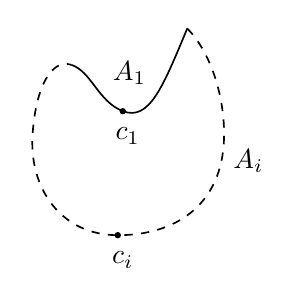
\begin{tikzpicture}[line width=0.6pt,scale=1.05]
  \draw[dashed] (0.32,1.32)
    .. controls (0.62,1.02) and (0.8,0.42) .. (0.76,-0.1)
    .. controls (0.7,-0.82) and (0.18,-1.18) .. (-0.52,-1.18)
    .. controls (-1.2,-1.18) and (-1.6,-0.62) .. (-1.55,0.05)
    .. controls (-1.51,0.62) and (-1.32,0.96) .. (-1.08,0.88);
  \draw (-1.08,0.88)
    .. controls (-0.84,0.8) and (-0.76,0.44) .. (-0.46,0.32)
    .. controls (-0.14,0.2) and (0.02,0.6) .. (0.32,1.32);
  \fill (-0.46,0.32) circle (1.1pt);
  \node at (-0.38,0.78) {$A_1$};
  \node at (-0.4,0.02) {$c_1$};
  \fill (-0.52,-1.18) circle (1.1pt);
  \node at (1.06,-0.28) {$A_i$};
  \node at (-0.46,-1.48) {$c_i$};
\end{tikzpicture}
\end{minipage}\hfill
\begin{minipage}[b]{0.46\textwidth}
\centering
\begin{tikzpicture}[line width=0.6pt,scale=1.05]
  \draw (-1.7,0.85)
    .. controls (-1.5,0.72) and (-1.1,0.48) .. (-0.75,0.3)
    .. controls (-0.4,0.12) and (-0.28,0.55) .. (0.05,1.3);
  \draw[dashed] (0.13,1.38)
    .. controls (0.42,0.95) and (0.72,0.25) .. (0.86,-0.35)
    .. controls (0.97,-0.78) and (0.97,-1.05) .. (0.9,-1.16)
    .. controls (0.83,-1.28) and (1.12,-1.32) .. (1.32,-0.95)
    .. controls (1.47,-0.6) and (1.63,0.5) .. (1.56,1.22);
  \fill (-0.75,0.3) circle (1.1pt);
  \node at (-0.66,0.76) {$A_1$};
  \node at (-0.68,0.0) {$c_1$};
  \fill (0.9,-1.16) circle (1.1pt);
  \node at (1.22,-0.24) {$A_i$};
  \node at (0.84,-1.46) {$c_i$};
\end{tikzpicture}
\end{minipage}
\caption{}
\label{fig:stable-manifold-closures}
\end{figure}

同样清楚地是，作为一个\trConnected{}空间的闭包，$A_i$ 是\trConnected{}的。显然，如果 $A_i$ 由 $W^s(c_i)$ 和单独一个点组成，那么后者是一个极大点，而 $A_i$ \trDiffeomorphic{}于一个\textbf{\trCircle}（circle）。同样地，如果 $A_i$ 由该\trStableManifold{}和添加上去的两个点组成，那么 $A_i$ \trDiffeomorphic{}于一个闭区间。

请注意，诸 $A_i$ 的并是整个 $V$：如果 $x\in V$，那么它的\trTrajectory{}趋于一个极小点，从而落在某一个\trStableManifold{}之中，除非 $x$ 是一个极大点，但这时它便落在某个\trStableManifold{}的闭包之中。

如果 $k=1$，那么该定理至此就已得证。否则，由于 $V$ 是\trConnected{}的，必存在一个 $i\ge 2$ 使得 $A_1\cap A_i\ne\varnothing$。这个交只含有局部极大点，因为唯有从这些点出发，我们才能下降到两个不同的极小点。特别地，$\partial V\cap(A_1\cap A_i)=\varnothing$。$A_1\cap A_i$ 中至多有两个点。我们有两种可能：
\begin{itemize}
\item 如果这个交含有两个点，那么这两个点都是极大点，$A_1\cup A_i$ \trDiffeomorphic{}于 $S^1$，于是大功告成。
\item 反之，如果它只含有一个点，那么 $A_1\cup A_i$ \trDiffeomorphic{}于 $[0,1]$。若 $A_1\cup A_i=V$，同样大功告成。
\end{itemize}
而如果情形并非如此，那么我们就继续把诸 $A_i$ 一个一个添上来，直到把它们用完为止。
\end{proof}

存在着这个定理的其他证明方式，它们也许更简单（参见 [55]）。这个使用\trMorse{}理论的证明，其优点在于为其他类似的证明做好了准备，例如\cref{thm:hm0-connected-manifold}的证明。

\subsection{一个应用：\trBrouwer\trFixedPoint{}定理}
\label{subsec:brouwer-fixed-point-theorem}

我们现在要利用\trSardTheorem{}以及我们关于维数为 $1$ 的\trManifold{}的知识，来证明\trBrouwer{}的那个著名定理（这个证明出自\trMilnor{}的书 [55]）。

\begin{theorem}\label{thm:brouwer-fixed-point}\BookIndexDefinition{T014}
设 $\varphi\colon D^n\to D^n$ 是一个连续映射；那么它有一个\trFixedPoint。
\end{theorem}

\begin{proof}
证明的第一部分在于化归到 $\varphi$ 为 $\cC^\infty$ 映射的情形；其细节我们在此不拟给出（参见 [45]）。接下来，从被假定是 $\cC^\infty$ 且没有\trFixedPoint{}的 $\varphi$ 出发，我们构造一个收缩
\[
r\colon D^n\longrightarrow S^{n-1}
\]
它把 $x\in D^n$ 送到\trSphere{} $S^{n-1}$ 与那条从 $\varphi(x)$ 出发且穿过 $x$ 的射线的交点。这样一来，如果 $x$ 是\trSphere{}上的一个点，它就原地不动。于是我们便得到一个在边界上限制为恒同映射的 $\cC^\infty$ 映射 $r$。\trSardTheorem{}断言，这个映射具有\trRegularValue。设 $a\in S^{n-1}$ 是其中的一个；那么 $r^{-1}(a)$ 是 $D^n$ 的一个维数为 $1$ 的\trSubmanifold，其边界为
\[
\partial r^{-1}(a)=r^{-1}(a)\cap\partial D^n=\{a\}\text{。}
\]
但是，一个维数为 $1$ 的\trManifoldWithBoundary{}\trDiffeomorphic{}于若干个\trCircle{}与闭区间之并，从而其边界由偶数个点组成。这就给出了一个矛盾，因而也就证明了\trFixedPoint{}的存在性。
\end{proof}
